%!TEX program = pdflatex
%# -*- coding: utf-8 -*-
%!TEX encoding = UTF-8 Unicode

\documentclass[12pt,oneside,a4paper]{article}
\usepackage{geometry}
\geometry{verbose,tmargin=1in,bmargin=1in,lmargin=1in,rmargin=1in}
\usepackage[pdfusetitle,
 bookmarks=true,bookmarksnumbered=true,bookmarksopen=true,bookmarksopenlevel=2,
 breaklinks=false,pdfborder={0 0 1},backref=false,colorlinks=false,
 unicode=true]
 {hyperref}
\hypersetup{pdfstartview={XYZ null null 1}}
\usepackage{url}
\setcounter{secnumdepth}{2}
\setcounter{tocdepth}{2}
\usepackage[final]{microtype}

\usepackage{amsmath, amsthm, amssymb, amsfonts}
\numberwithin{equation}{section}
\usepackage[retainorgcmds]{IEEEtrantools}
\usepackage{bm}

\usepackage[T1]{fontenc}
\usepackage[utf8]{inputenc}
\usepackage[lf]{MinionPro}
\usepackage[toc,eqno,enum,bib,lineno]{tabfigures}
\usepackage{etoolbox}
\AtBeginEnvironment{tabular}{%
    \figureversion{tab}
}
\linespread{1.3}
\setlength{\parskip}{.5\baselineskip}

\usepackage{graphics}
\usepackage{graphicx}
\usepackage{subcaption}
\usepackage[figure]{hypcap}
\usepackage[font=normalsize, tableposition=above]{caption}
% \usepackage{tikz}
% \usepackage{tikz-cd}
%\usepackage{grffile}
%\usepackage{float}
\usepackage{pdfpages}
\usepackage{pdflscape}

\usepackage{multirow}
\usepackage{booktabs}
\usepackage{threeparttable}
\usepackage{dcolumn}

%\usepackage[square,numbers,super,comma,sort]{natbib}
\usepackage[backend=biber, style=nature, sorting=none, isbn=false, url=false, doi=false]{biblatex}
\addbibresource{ref.bib}
\usepackage[]{authblk}

\usepackage{verbatim}
\usepackage{fancyvrb}

\usepackage{fancyhdr}
\pagestyle{fancy}
\usepackage{extramarks}
\usepackage{lineno}

\newcommand{\hmwkTitle}{Learning to Classify PC Malwares}
\newcommand{\hmwkAuthorName}{Jingxiang Li\\Advisor: Yuhong Yang}

\lhead{Jingxiang Li, Advisor: Yuhong Yang}
\chead{}
\rhead{\hmwkTitle}
\cfoot{\thepage}

\setlength\headheight{15pt}
\setlength\parindent{0pt}

\newcommand{\m}[1]{\texttt{{#1}}}
\newcommand{\E}[0]{\mathrm{E}}
\newcommand{\Var}[0]{\mathrm{Var}}
\newcommand{\sd}[0]{\mathrm{sd}}
\newcommand{\Cov}[0]{\mathrm{Cov}}

\title{\hmwkTitle}
\author{\hmwkAuthorName}
\date{}


\begin{document}
\maketitle

\begin{abstract}
Malware, short for``malicious software'', is defined as the kind of computer software that can be used to intentionally cause damage to computer hardware, disrupt the function of operation systems, illegally gather private information, or display unwanted advertising. Every single day there are 390,000 new malware families being reported and registered, hence malware detection programs are becoming more than important to prevent attacks from millions kinds of malware. One challenge in the design of malware detection system is to categorize malware variants into their families. In this article, an end-to-end malware classification framework is proposed to address this problem. In the framework, we first disassemble malicious executables to obtain their assembly code, then features will be scanned and extracted from it, including text features, image features, and meta data features. Next, n-grams, tf-idf, singular value decomposition, principal component analysis and Random Forest will be applied for dimensionality reduction and selection. After feature engineering, 500 important features are founded and used for further predictive modeling. In order to build capable malware classifier, machine learning techniques are applied to learn classification rules. Several candidate models are evaluated and compared based on a newly released dataset, where 8 malware families are included. The best model we built successfully achieve 97\% total accuracy, and show superior performance on other metrics, suggesting that our framework is capable enough and can definitely be utilized as part of the malware detection software.
\end{abstract}

\thispagestyle{empty}
\clearpage

\tableofcontents
\clearpage

\renewcommand\baselinestretch{1.5}\selectfont
\section{Introduction}
Malware, short for``malicious software'', is defined as the kind of computer softwares that can be used to intentionally cause damage to computer hardwares, disrupt the function of operation systems, illegally gather private information, or display unwanted advertising. There does not exists an official definition for explaining what malware is, but basically malware can be thought of as computer software or program whose objective is malevolent, as mentioned by Christodorescu \cite{christodorescu2005semantics}.

According to the research from AV-TEST institute \cite{avtest}, the total number of malware families is approaching 600,000,000, and every single day there are 390,000 new malware families being reported and registered. More than that, the number of new malwares families being discovered is increasing exponentially from the year 2006, suggesting that malwares are becoming the biggest threat for everyone on the Internet, not only individuals, but also companies, even governments. For individuals, malwares can steal their passwords, gather private information like full name, date of birth, social security number, mailing address, telephone address, and sell them to the market or criminals. For companies and governments, their data can be stolen or tampered, which may cause great security issue and cost them huge amount of money and time in order to fix it. Therefore, malware detection programs are becoming more than important to prevent attacks from millions kinds of malware.

Knowing that malware detection is critical to everyone on the Internet, establishing effective malware detection system is actually a challenging work to do because in most cases malwares are designed to operate undetected. Common techniques for operating undetected include: Viruses, Trojan Horses, Rootkits, etc. Before 2015, the pattern of malwares are easy to define and hence malware detection can be done simply by scanning specific signatures of programs. For example, anti-virus programs can detect most of malwares by scanning the first several bits of the target file and match them to the malware database. However, since the beginning of 2015, many new techniques and their combinations are applied to malwares and make them difficult for detection. this kind of malware is called evasive malware \cite{evasive}, which utilizes tricks to evade detection from old anti-malware programs. For example, for the purpose of evading detection, malware authors may apply polymorphism to the malevolent components. In this way, malicious files belonging to the same malware family can be constantly modified or obfuscated using various techniques, so that they look like different files with different functionalities. Therefore, classifying malwares has become one of the greatest challenge in the design of malware detection system. In order to classify evasive malwares, new approaches that are capable to find and utilize more complicated patterns must be introduced and applied. In this article, a machine learning based framework will be proposed to analyze the contents of malicious software and make accurate classification.

Machine learning techniques have attracted tremendous attentions in recent years. Many of techniques have been applied in various of industries and yielded great success. McGrattan defined machine learning as a ``field of study that gives computers the ability to learn without being explicitly programmed'' \cite{mcgrattan1999maintenance}, which means that instead of manually construct solutions, machine learning techniques try to solve problems by learning patterns from data. For example, in order to distinguish malwares from innocent files, instead of explicitly program the patterns of malwares, machine learning techniques are capable to build models to learn the difference between malwares and innocent files given labeled files, and then use the pattern they learned to make prediction for new files need to be classified. The advantage of machine learning techniques over traditional approaches is that, researchers do not have to manually construct complicated rules for classification, they can use algorithms to automatically learn the rules from data. In most cases, human-beings are not capable to understand a complicated system, but machine learning algorithms have their way to learn useful patterns. This is the reason that we choose machine learning techniques for malware detection and classification, where explicitly defining rules is almost impossible especially for evasive malwares.

Though machine learning techniques are powerful for classification and prediction, they require big amount of data and carefully selected features to be used to learn the pattern. Since there are so many malwares reported everyday, the amount of data may not be an issue in the construction of malware detection system. However, features are difficult to define in this area, because malwares are simply softwares, they are hard to be vectorized in a reasonable way. Therefore feature engineering become one of the most critical parts for machine learning based malware detection modeling. There are two common ways to extract features from malicious softwares, by static analysis or by dynamic analysis. Static analysis means to find features by analyzing the content of malwares, in most cases the source code or the hexadecimal representation of the malwares. By static analysis features can be defined as the frequency of function calls, library links, variables, registers, operation code, etc. Techniques in natural language processing, like n-grams and topic model, can also be applied to extract more meaningful features. Hence it is relatively easier to build machine learning models based on static analysis. For dynamic analysis, malwares will be executed in a sandbox and their behaviors will be counted as features for learning. Though dynamic analysis might be a more direct approach for malware detection, obviously collecting features from dynamic analysis is more difficult than that from static analysis, and will cost a great amount of extra money and time. For this reason, we prefer static analysis in this article and will apply machine learning models based on features extracted from the contents of malwares.

The idea of applying machine learning techniques in malware detection can be traced back to the year 1996 when Tesauro and his team developed an artificial neural network for generic detection of a particular class of computer viruses -- the so called boot sector viruses that infect the boot sector of a floppy disk or a hard drive \cite{tesauro1996neural}. In the article they announced that they deployed their neural network as a commercial product as part of IBM Anti-virus software package. They applied trigrams to extract features from the byte strings of computer malwares and then use it as the input of their artificial neural network. They collect on 200 viral examples and 100 non- viral examples as the entire dataset, and use half of them for training, half for testing. The performance on the test set is about 80\% to 85\% accuracy for viral examples, and 100\% for legitimate examples, which is a great success at that time. They further control the false discovery rate of their artificial neural network by lifting up the threshold used for classification. In 2001 Schultz ans his team proposed their data mining approaches to detect new, previously unseen malicious executables accurately and automatically \cite{schultz2001data}. In the dataset there are 4,266 programs split into 3,265 malicious binaries and 1,001 clean programs. They collected features in three main categories: 1. Dynamically Linked Libraries (DLL), 2. GNU strings, and 3. byte sequence using hexadecimal representation of malwares. In modeling, they choose Naive Bayes and Multi Naive Bayes for classification and prediction, and further compare it with some other techniques. As the result, Both Naive Bayes classifiers achieve around 97\% total accuracy, which outperforms traditional approaches significantly. In 2006, Kolter and Maloof describe the use of machine learning and data mining to detect and classify malicious executables as they appear in the wild \cite{kolter2006learning}. They applied various machine learning techniques to differentiate malwares from benign executables, and compare them based on multiple model evaluation measures. 1,971 benign executables and 1,651 malicious programs are included in the dataset. They applied n-grams on the byte code of programs followed by a feature selection procedure to extract features for modeling. They evaluated a number of machine learning algorithms in this problem, including Naive Bayes, decision trees, support vector machine and boosting method. As the result, boosting trees dominated other classifiers with AUC of 0.996, almost a perfect performance in terms of prediction. They also evaluated their model on 291 new malwares that are collected after their original gathering, and the model they chose achieved 0.98 true positive rate along with a 0.06 false positive rate. This result further confirmed their thought that the model they built can be used for the establishment of modern malware detection systems. In 2011, Rieck et al. proposed a general framework for automatic analysis of malware behavior using machine learning \cite{rieck2011automatic}. The framework applied both clustering and classification techniques in order to identify novel families of malwares and make decisions for malware detection. They also proposed a incremental analysis procedure that further improve the efficiency of their behavior based analysis. They announced that the incremental analysis they proposed can significantly reduce the run-time overhead of their methods, while providing sufficient accuracy for novel malware variants. In 2012, Sahs and Khan proposed their kernel based approach to Android malware detection \cite{sahs2012machine}. They extract features from the requested permissions of APK and the control flow graph constructed from the raw byte representation of APK. Then kernels for string and graph are carefully designed and applied along with the one class support vector machine for novel malware detection. They evaluate their malware detection system based on a collection of 2081 benign programs and 91 malicious softwares. As the result, the system yielded a reasonable false discover rate, but performed poorly in discrimination. In 2013 Dahl et al. proposed their large-scale machine learning classification framework using random projections and neural networks \cite{dahl2013large}. The goal of their framework is to achieve an extremely low false positive rate (less than 0.01\%) with a reasonably low false negative rate (less 5\%). They collected over 2.6 million files, 1,843,359 of which are malicious and 817,485 of which are benign. For feature engineering, they extracted three types of features including null-terminated patterns observed in the process' memory, tri-grams of system API calls, and distinct combinations of a single system API call and one input parameter. After that random projection and feature selection were applied to reduce the dimension of features. As the result there are around 179 thousand features selected for training the malware detector. logistic regression and artificial neural networks with various structures are applied for classification modeling. As the result, the two class error rate is about 0.5\%, with false positive rate around 0.9\% and false negative rate around 0.3\%. Rather than analyzing the malwares as sequences of bytes or system API calls, Nataraj et al. try visualize malware's contents and then construct models based on the so called ``malware image'' \cite{nataraj2011malware}. Nataraj et al. visualize the malware binaries as gray-scale images, where adjacent two hexadecimal points can be transformed to a gray-scale point from value 0 to 255. After that, GIST was applied to extract features from malware images, and classification model (k-nearest neighbor classifier) was trained based on the GIST features. This malware classification framework was evaluated on a dataset consisting of 8 malware families and totaling 1713 malware images. As the result, their malware image based framework yielded great success with the total classification accuracy of 0.9929 and standard deviation of 0.002.

Inspired by the above researches, in this article we will propose a comprehensive framework for malware detection or classification. Our framework will combine information from various sources, like byte sequence, operation code sequence, malware image and more. Then, modern machine learning techniques will be applied for dimension reduction and predictive modeling. The capability of our model will be evaluated in a newly released dataset. We will show that our framework is capable enough and can be utilized as part of the malware detection softwares.

\clearpage
\section{Background}
In order to construct machine learning models for analyzing and classifying malwares, it is important to have basic understanding about computer programs. The knowledge in structure and execution of computer programs will be the key determinants for feature engineering in the modeling procedure. In most cases, a computer software would be generated in the following steps, 1. Programmers write the code in a programming language (for example C), 2. The corresponding compiler generates assembly code versions of the software, 3. The assembler converts the assembly code into binary object-code files, which contains binary representations of all instructions. 4. The linker merges object-code files and shared libraries together and generates the executables \cite{bryant2003computer}. In malware detection, the only thing we have on hand would be executables. However, it would be very challenging if we try to directly analyze executables, because they are just a sequence of binary numbers, we will lose a lot of information by only looking at the binary representation of the executables. Therefore, it would be better if we can analyze the assembly code of executables, since we can extract information like instructions from the assembly code. For 32 bit executables in Microsoft Windows system, Interactive Disassembler (IDA) is a powerful tool to disassemble executables to their assembly code. For example, the following are some segments of assembly codes converted from a malware:

\begin{Verbatim}[fontsize=\small]
.text:00401090 8B 44 24 10    mov     eax, [esp+10h]
.text:00401094 8B 4C 24 0C    mov     ecx, [esp+0Ch]
.text:00401098 8B 54 24 08    mov     edx, [esp+8]
.text:0040109C 56             push    esi
.text:0040109D 8B 74 24 08    mov     esi, [esp+8]

......

.idata:005265CC               ; Imports from WS2_32.dll
.idata:005265CC               ;
.idata:005265D0               ; int __stdcall WSACleanup()
.idata:005265D0 ?? ?? ?? ??   extrn WSACleanup:dword  ; CODE XREF: _WinMain@16_0+
.idata:005265D0               ; DATA XREF: _WinMain@16_0+
\end{Verbatim}

From the above code segments we can clearly see the way how the malware is organized. For each line of the assembly code, they are: 1. Code segments (e.g. .text, .idata), 2. Memory address of the line of code (e.g. 00401090), 3. Binary representation of the code (e.g. 8B 44 24 10), 4. Operation code (opcode) defined as a single instruction executed by the CPU (e.g. mov), 5. Operands (e.g. eax, [esp+10h]), 6. Dynamic link libraries imported to the program (e.g. WS2\_32.dll), 7. Function called by the program (e.g. WSACleanup). The structure of this kind of assembly code is clear, therefore extracting information from it is easier than extracting information from pure binary representations.

\clearpage
\section{Data Description}
To evaluate the performance of our proposed machine learning based malware classification framework, we will test it on a newly released dataset from Microsoft \cite{microsoft}. The dataset is originally released for a Kaggle competition, named Microsoft Malware Classification Challenge (BIG 2015), whose purpose is to encourage open sourced solutions and techniques for grouping variants of malware files into their respective families. There are 9 families of malwares included in the dataset, they are 1. Ramnit, 2. Lollipop, 3. Kelihos\_ver3, 4. Vundo, 5. Simda, 6. Tracur, 7. Kelihos\_ver1, 8. Obfuscator.ACY, 9. Gatak. All of them are powerful malwares that broadly spread over millions of computers. More than 10 million individuals were influenced by these malwares. We will apply our malware classification framework on this dataset to accurately classify any given malware and determine which family it belongs to.

In the dataset, there are totaling 10,868 malwares including 1541 variants of Ramnit, 2478 of Lollipop, 2942 of Kelihos\_ver3, 475 of Vundo, 42 of Simda, 751 of Tracur, 398 of Kelihos\_ver1, 1228 of Obfuscator.ACY and 1013 variants of Gatak. Compared to other malware families, the sample size of class 5 Simba is so limited that it is very likely to cause great influence to the final classification result, hence we decided to ignore this kind of malwares from the dataset. Therefore there will be \textbf{10,826 malwares} included in the dataset we are analyzing, with \textbf{8 families} to be classified. All malwares are well labeled, hence we can train our models on one subset and evaluate their performances on another disjoint subset to get an unbiased estimate for the measure of predictive capability. Here in this article, we applied a stratified randomized sampling strategy to split the dataset into two disjoint parts, one with 5\% malwares as the training set and another one with 95\% malwares as the test set. The reason that we choose such a small subset to train models is to enlarge the differnces among different classifiers, so it becomes more convenient for us to determine which model is the best one. In summary, there will be 542 malware variants in the training set, 10284 of them in the test set. Since stratified random sampling is applied, the distribution of malware families are ensured to be very close in both subsets, which is very important for obtaining an unbiased predictive measure of our malware classification framework.

Note that the numbers of malware variants in each family are different, suggesting that classifiers without adjustment for unbalanced dataset are very likely to show great bias to families with large sample size. Hence techniques that are capable to handle unbalanced dataset should be used in solving this problem. There might be outliers in the dataset because not all malwares are disassembled correctly from IDA. However, the number of outliers should be very small. It would be better if we can choose classifiers that is not very sensitive to outliers.

For each malware there are two associated text files. One has suffix ``.bytes'', which is the hexadecimal representation of the malware executable; the other has suffix ``.asm'', which is the assembly code disassembled by Microsoft's Interactive Disassembler (IDA). Note that the binary representations in the ``.bytes'' file are exactly the same as what we can find in the corresponding ``.asm'' file, i.e. they are simply different representations for the same variant of computer malware. In this article, we are going to analyze the contents from these two files in a static manner and construct our malware classification framework. Here we provide an example text files for a malicious malware coded as ``0A32eTdBKayjCWhZqDOQ''.

\begin{Verbatim}[fontsize=\small]
0A32eTdBKayjCWhZqDOQ.asm
.text:00401060 8B 44 24 08      mov     eax, [esp+8]
.text:00401064 8A 08            mov     cl, [eax]
.text:00401066 8B 54 24 04      mov     edx, [esp+4]
.text:0040106A 88 0A            mov     [edx], cl
.text:0040106C C3               retn
.text:0040106D CC CC CC         align 10h
.text:0040106C                  ; ---------------------------------------------------------------------------
.text:00401070 8B 44 24 04      mov     eax, [esp+4]
.text:00401074 8D 50 01         lea     edx, [eax+1]
.text:00401077
.text:00401077                  loc_401077:   ; CODE XREF: .text:0040107
.text:00401077 8A 08            mov     cl, [eax]
.text:00401079 40               inc     eax
.text:0040107A 84 C9            test    cl, cl
.text:0040107C 75 F9            jnz     short loc_401077
.text:0040107E 2B C2            sub     eax, edx
.text:00401080 C3               retn

\end{Verbatim}
\begin{Verbatim}
0A32eTdBKayjCWhZqDOQ.bytes
00401060 8B 44 24 08 8A 08 8B 54 24 04 88 0A C3 CC CC CC
00401070 8B 44 24 04 8D 50 01 8A 08 40 84 C9 75 F9 2B C2
\end{Verbatim}

The above code segments provide two representations for contents with the same memory address. Here we could see that the binary representations in the ``.bytes'' file are exactly the same as the hexadecimal sequence in the ``.asm'' file. The reason two representations are provided is that some of the segments in ``.asm'' file are collapsed, for example the ``.rsrc'' and the ``.reloc'' segments. They are collapsed to make sure that the size of the ``.asm'' file is reasonable. However, code in these segments can be found in the ``.bytes'' file.

\clearpage
\section{Evaluation Metrics}
In this section several evaluation metrics for multi-class classification tasks will be introduced, for evaluating the generalization performance of our malware classification framework. As a classification problem, we would like to measure both the global classification performance over all classes and performance on each single malware family. In this way, not only the overall capability of our malware classification framework can be estimated, we can also inspect its performance in detail and research directions for further improvement.

First, for the measuring of the global classification performance, we choose the following two metrics: \textbf{negative multi-class logarithmic loss (logloss)} and \textbf{accuracy score}.

Multi-class logarithmic loss function is defined as:
\begin{equation}
\mathrm{logloss} = -\frac{1}{N}\sum_{i = 1}^{N}\sum_{j = 1}^{M}y_{ij} \log(p_{ij})
\end{equation}
Where $N$ is the sample size in the test set, $M$ is the number of labels. $y_{ij} = 1$ if observation $i$ belongs to class $j$ and $0$ otherwise. $p_{ij}$ is the predicted probability that observation $i$ belongs to class $j$. For mathematical convenience, the predicted probability will be replaced by
$$\max(\min(p, 1 - 10^{-15}), 10^{-15})$$
in order to avoid the influence of extreme large values. Note that probability output is required for multi-class logarithmic loss function, hence classifiers like Support Vector Machine (SVM) cannot be applied directly to this problem. Further probability calibration will be needed if SVM were expected to deploy.

Accuracy score is defined as:
\begin{equation}
\mathrm{Accuracy = 1 - \frac{\# \mathrm{misclassified}}{N}}
\end{equation}
where $\#\mathrm{misclassified}$ indicates the number of observations being misclassified by the model. This measure does not require probability output, hence it is less sensitive than the multi-class logarithmic loss.

Next, in order to measure the model's generalization performance on each specific malware family, we will apply an one versus the rest strategy and calculate the \textbf{Recall, Precision and $\mathbf{F_{1}}$} score for each of them. In the one versus the rest strategy, the malware family we are focusing on will be treated as positive observations, along with all others being treated as negative observations. Then, by constructing confusion matrix for each malware family, Recall, Precision and $F_{1}$ score can be obtained using the following formulas:
\begin{equation}
\mathrm{Recall} = \frac{\mathrm{TP}}{\mathrm{TP} + \mathrm{FN}}
\end{equation}
\begin{equation}
\mathrm{Precision} = \frac{\mathrm{TP}}{\mathrm{TP} + \mathrm{FP}}
\end{equation}
\begin{equation}
F_{1} = 2 \cdot \frac{\mathrm{Precision} \cdot \mathrm{Recall}}{\mathrm{Precision} + \mathrm{Recall}}
\end{equation}

Where TP indicates the True Positives, FN indicates False Negatives, FP indicates False Positives. Note that Recall is just the true positive rate which measures how well the model can do to find correct positive instances. Precision is closely related to the false discovery rate (FDR), where $\mathrm{Precision} = 1 - \mathrm{FDR}$. $F_{1}$ score is simply the harmonic mean of precision and recall, therefore $F_{1}$ score can be interpreted as a comprehensive metric that measures the prediction performance on positive observations, by combining the information from Recall and Precision. These three metrics are widely applied in fields like information retrieval, text classification and cancer diagnosis. Fujino et al. proposed a framework for multi-label text categorization by directly maximize $F_{1}$ score on model combination \cite{fujino2008multi}; Ritter et al. applied $F_{1}$ score to evaluate their models for named entity recognition in tweets \cite{ritter2011named}; Petrovic used the same measure to evaluate their histology images based deep neural networks in mitosis detection in breast cancer \cite{cirecsan2013mitosis}. In this article, $F_{1}$ score, along with Recall and Precision, will be reported and compared for all classification models.

\clearpage
\section{Feature Engineering}
In this section we will introduce the way we extract features from the disassembled files of malicious software. In our framework, we collected features from 4 categories:
\begin{enumerate}
  \item Text features from ``.asm'' file
  \item Text features from ``.bytes'' file
  \item Image features from ``.bytes'' file
  \item Meta data features from both ``.asm'' file and ``.bytes'' file
\end{enumerate}
The entire feature engineering process can be visualized in diagram \ref{feature engineering}.
\begin{figure}[ht!]
\centering
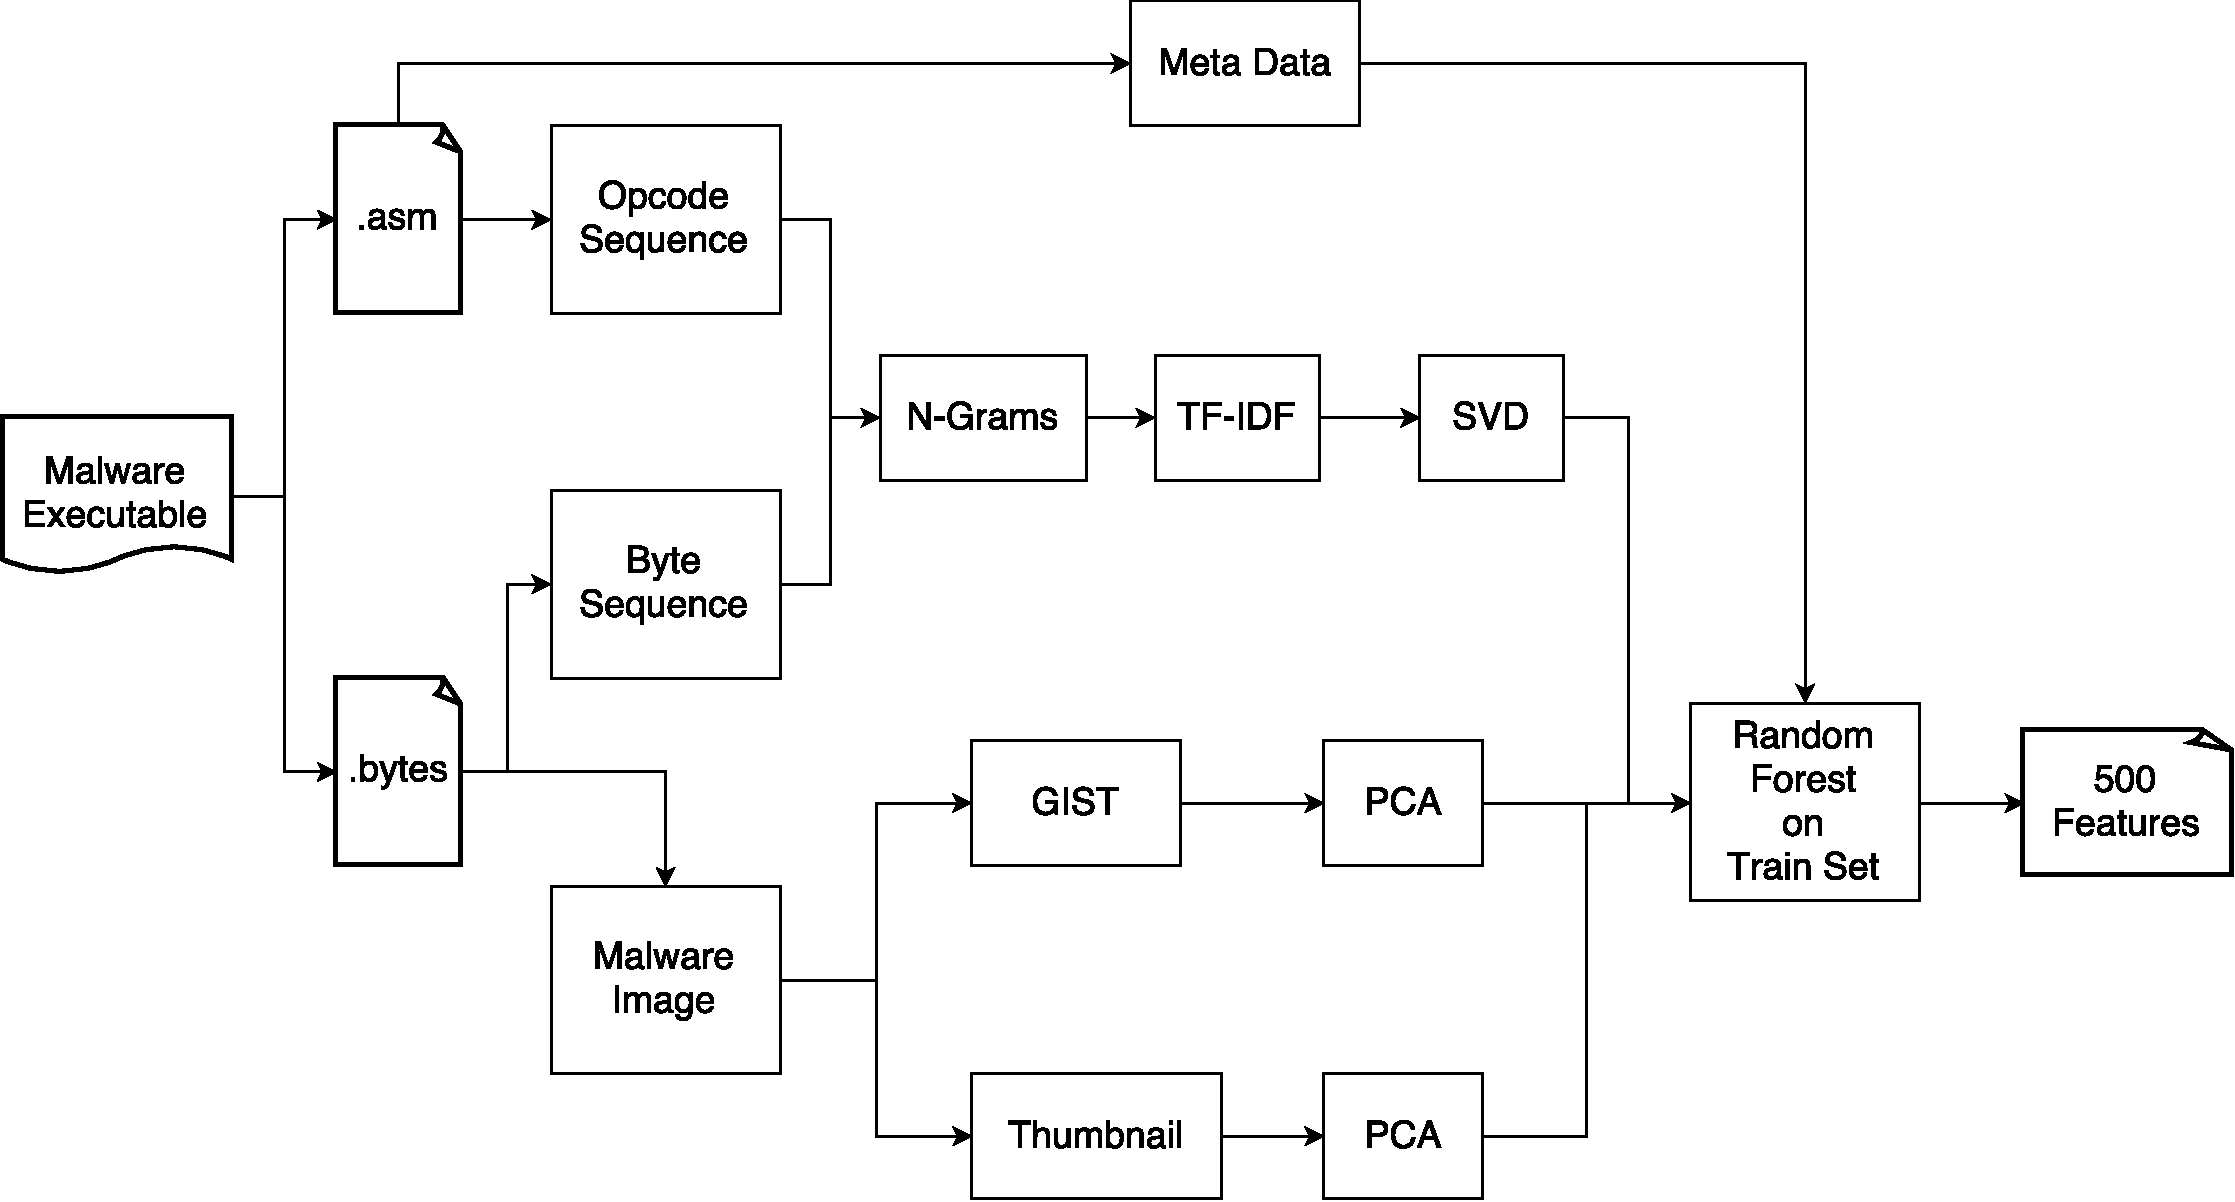
\includegraphics[width=.9\linewidth]{./imgs/FeatureEngineering.pdf}
\caption{The Feature Engineering Process}
\label{feature engineering}
\end{figure}

Next we will explain each step in the feature engineering process in detail.

\subsection{Text features from ``.asm'' file}
For features in the ``.asm'' file, we mainly focus on the Operation Code, i.e. Opcode. An Opcode is a single instruction that can be executed by the CPU, hence sequence of Opcode contains almost all information about how the program be executed and its behavior. By applying analysis on sequence of Opcode, we are very likely to find useful patterns for malware classification. Thanks for the structured output from IDA, we can easily extract all Opcodes from the ``.asm'' file using regular expression. Here is an example showing the Opcode sequence extracted from a code segment in an ``.asm'' file.

\begin{verbatim}
.text:00401310 8B 4C 24 04           mov     ecx, [esp+4]
.text:00401314 B8 1F CD 98 AE        mov     eax, 0AE98CD1Fh
.text:00401319 F7 E1                 mul     ecx
.text:0040131B C1 EA 1E              shr     edx, 1Eh
.text:0040131E 69 D2 FA C9 D6 5D     imul    edx, 5DD6C9FAh
.text:00401324 56                    push    esi

Opcode Sequence: mov, mov, mul, shr, imul, push
\end{verbatim}

Once opcode sequences are collected from all malware variants in the dataset, we apply the following procedure to get vectorized features from each sequence:
\begin{enumerate}
  \item Extract word n-grams (n = 1, 2, 3, 4) from the opcode sequence and construct 4 feature sets corresponding to the 4 kinds of n-gram models
  \item Apply normalized TF-IDF transformation on each feature set
  \item Apply Singular Value Decomposition on each feature set for dimension reduction
  \item Concatenate four feature sets together
\end{enumerate}

While Opcode sequences are extracted for all malware variants, n-gram is applied to get vectorized features from sequences. n-gram word features are frequencies of all subsequences of length n. The idea for using n-gram features came from Tony et al. where n-gram signatures are applied for the detection of new malicious code \cite{abou2004n}. Same technique is also applied in multiple areas associated with sequence analysis, for example, Ganapathiraju et al. applied n-gram model to analyze the whole-genome protein sequences \cite{ganapathiraju2002comparative}; Lo et al. proposed a n-gram system that is capable to automatically generate music sequence. Therefore it is reasonable for us to apply n-gram to model the Opcode sequence in this problem. In our framework, we extract 1-gram, bi-gram, tri-gram and four-gram as features. After that, we notice that there are more than 20 thousands of n-grams are extracted, hence we are going to filter them using a simple approach to eliminate n-grams with negligible frequency. For 1-gram and bi-gram features, we include those which appear more than 150 times in at least one malware files; for 3-gram and 4-gram features, we only select those which appear more than 100 times in at least one malware files. We construct 4 different feature set corresponding to the 4 kinds of n-gram models.

After that, normalized TF-IDF transformation is applied on each feature set. TF-IDF, short for Term Frequency Inverse Document Frequency, is a numerical statistic that measure the relevance of a word is to a document in a corpus. Words with high TF-IDF numbers imply a strong relationship with the document they appear in, suggesting that if that word were to appear in a query, the document could be of interest to the user \cite{aizawa2003information}. Let $t$ be the term or word, $d$ be the document, $D$ be the corpus, $|\{\cdot\}|$ be the cardinality of a set, then
\begin{equation}
  \mathrm{TF-IDF(t, d, D) = \mathrm{tf}(t, d) \cdot (\mathrm{idf}(t, D)} + 1)
\end{equation}
where
$$\mathrm{tf}(t, d) = |\{t \in d\}|$$
$$\mathrm{idf}(t, D) = \log \frac{|\{d \in D\}|}{|\{d \in D : t \in d\}|}$$
Here we could see that TF is just the word count in one document which measures the importance of the word in that document, and IDF is an inverse proportion of the document that contains the word, which measures how rare the word term is in the corpus. By combining these two measures together, TF-IDF is capable to measure to relevance of word in each document for a given corpus. In malware classification, we define Opcode as word, Opcode sequence as document and the whole malware dataset as the corpus, therefore TF-IDF can be naturally applied on the n-gram feature sets we just get in the last step. After getting the TF-IDF transformed feature set, each row of the set will be normalized to make sure that the 2-norm of each row is 1.

Notice that after these two steps, the dimension of feature sets are still high (more than 10,000). Since we only have no more than 7,000 malware variants in the training set, dimension reduction techniques have to be applied in this problem. Here we use Singular Value Decomposition (SVD) to reduce the dimension of our feature set. SVD is a kind of matrix factorization method. For a $m \times n$ matrix $M$, it can be factorized in the form $M = U \Sigma V^{T}$, where $U$ is a $m \times m$ orthogonal matrix, $V$ is a $n \times n$ orthogonal matrix, $\Sigma$ is a $m \times n$ rectangular diagonal matrix with non-negative values on the diagonal. By SVD, we can use Matrix $M$ as the feature set for effective dimension reduction. The reason that SVD make sense in this problem is that, the factorized matrices can be explained as a topic model in natural language processing \cite{l2010latent}. $U$ can be viewed as a matrix with document's weight on topics, $V$ can be interpreted as a matrix with word's weight on topics, $\Sigma$ is the weight of topics in the corpus. Hence by SVD, we can extract topic vectors from the TF-IDF feature set and accomplish dimension reduction. For choosing the number of target dimensions, we simply choose $n$ components such that the variance explained by these $n$ components can achieve 95\%. It can be easily calculated from the $\Sigma$ matrix.

After dimension reduction, the four feature sets will be concatenated together for further processing.

\subsection{Text features from ``.bytes'' file}
Similar to what we did in the ``.asm'' file, we also extract features from the byte sequences in the ``.bytes'' file. We view each two adjacent hexadecimal numbers as a single word, and consider 1-gram, bi-gram and 4-gram subsequences as features. TF-IDF and SVD will also be applied for relevance transformation and dimension reduction.

\subsection{Image features from ``.bytes'' file}
Inspired by Nataraj's work, we decide to visualize malware as gray-scale images and see if features can be extracted by some image processing techniques. To construct gray-scale malware image, we simply treat every adjacent two hexadecimal numbers as a single number from 0 to 255 as gray-scale value, and then reshape this number sequence to an image. To determine the width of the image, we use the following criteria: 1. The width of the image should be a 16 times an integer number, 2. The width and the length should be as close as possible, 3. additional gray-scale values should be discarded. In this way we can easily visualize each malware as a gray-scale picture. Here some sample images from malware family Lollipop and Obfuscator.ACY are provided in figure \ref{malware image lollipop} and figure \ref{malware image Obfuscator}, where we could see significant difference in the textures of images. There exists clear vertical pattern in Lollipop images, and great amount of blackness can be found in the Obfuscator.ACY images. Therefore analyzing the texture pattern of malware images are very likely to help build an accurate malware classification model.

In order to extract features from the model, we apply GIST descriptors, which is an global descriptors for constructing a low dimensional representation of images \cite{oliva2001modeling}. GIST descriptors have been successfully applied in problems like scene classification and image categorization. Given a image, the GIST descriptor is calculated by the following steps: First, convolve the image with 20 pre-designed Gabor filters to construct 20 feature maps. Then divide each feature map into 16 regions (by a $4 \times 4$ grid), and then average the feature values within each region. At last, concatenate the 16 averaged values of all 20 feature maps, resulting in a $16 \times 20 = 320$ GIST descriptor, which is simply a vector with length 320. More than that, we also include a $16 \times 16$ image thumbnails into the feature vector. Principal Component Analysis will be applied to both of two feature sets for dimension reduction.

\subsection{Meta data features from both ``.asm'' file and ``.bytes'' file}
We also include meta data features in our analysis, that include:
\begin{enumerate}
  \item Segment count from ``.asm'' file
  \item file size for ``.asm'' file
  \item file size for ``.bytes'' file
\end{enumerate}
These features are considered to be useful in building the malware classification model and hence will be appended to our feature set.

After concatenating all features from different sources, Random Forest will be applied for further dimension reduction. We will simply train a Random Forest model on the training set and select the top 500 features based on the estimated feature importance. Therefore, only 500 important features will be included in the final predictive modeling procedure.

Here we applied a dimensionality reduction model called t-Distributed Stochastic Neighbor Embedding (t-SNE) to visualize our dataset in a 2-dimensional space. t-SNE, proposed by Maaten and Hinton, is a prize wining dimensionality reduction tool that is particularly well suited for the visualization of high-dimensional data \cite{maaten2008visualizing}. The advantage of t-SNE over traditional approaches like PCA, SVD is that, t-SNE preserve the neighborhood information among all observations, and hence t-SNE is more likely to generate reasonable low-dimensional representation for high-dimensional data. Figure \ref{t-sne} shows our data in a 2-dimensional space, each color indicates an malware family. As what has been shown in the figure, on the left hand side we can see clear separate malware clusters formed by malware variants in the same family. On the right hand side, Though clusters of observations are not well separated, malware variants in the same family still show tendency to group together. The t-SNE graph suggests that features, extracted from our feature engineering procedure, have great potential and possibility to serve as the base for further malware classification.

\begin{figure}[htbp]
\centering
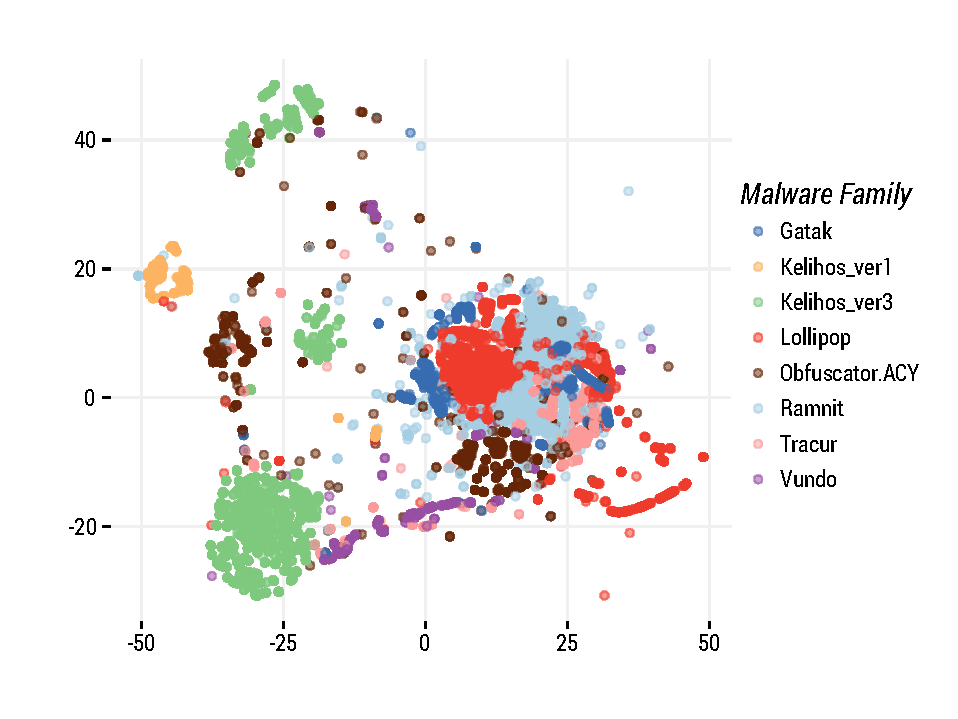
\includegraphics[width=.9\linewidth]{./imgs/tsne.pdf}
\caption{t-SNE Visualization with 500 Selected Features}
\label{t-sne}
\end{figure}

\clearpage
\section{Predictive Modeling}
After obtaining the entire feature set, we apply various of classifiers to train a predictive model for discriminating malware variants into families. We choose the following classifiers to finish our malware classification framework:
\begin{enumerate}
  \item Naive Bayes (NB)
  \item Multinomial Logistic Regression (Multi-Logreg)
  \item One-vs-Rest Logistic Regression (OvR-Logreg)
  \item Linear Discriminant Analysis (LDA)
  \item Quadratic Discriminant Analysis (QDA)
  \item Support Vector Machine with Probability Calibration (SVM)
  \item Random Forest Classifier (RF)
  \item Extremely randomized trees (ExtraTrees)
  \item eXtreme Gradient Boosting (XGBoost)
\end{enumerate}
We will try all these models and compare their performances based on evaluation metrics introduced before. In order to build models with optimal hyper-parameters and obtain unbiased estimates for their generalization power, we will use the following modeling procedure:
\begin{enumerate}
  \item Construct a set of hyper-parameter settings
  \item Randomly select a hyper-parameter setting from the set
  \item Validate model's performance by stratified 5-fold cross-validation
  \item Repeat process 1 to 3 several times
  \item Find the hyper-parameter setting that gives the best performance on cross-validation, retrain the model with that setting
  \item Evaluate the performance of this model on the test set, and record measures
\end{enumerate}
We will repeat this procedure 10 times and use the averaged measure to estimate model's generalization capability. The standard deviation of those metrics will also be used to quantify the robustness of the model. Next we will give a brief introduction about the machine learning algorithms mentioned in this section.

\subsection{Naive Bayes}
Naive Bayes is the kind of classifier that directly apply the Bayes' theorem with ``naive'' assumption of independence among any components of feature vectors. It has been successfully applied in areas like email filtering \cite{mccallum1998comparison} and rRNA sequence analysis \cite{wang2007naive}.  Here we will see its performance on malware classification. Given a set of features $x_{1}$ through $x_{n}$ and the class label $y$, Bayes' theorem tells that
\begin{equation}
P(y | x_{1}, x_{2}, \dots, x_{n}) = \frac{P(y) P(x_{1}, x_{2}, \dots, x_{n} | y)}{P(x_{1}, x_{2}, \dots, x_{n})}
\end{equation}
Due to the assumption that features are independent with each other, we have
\begin{equation}
P(x_{1}, x_{2}, \dots, x_{n} | y) = \prod_{i = 1}^{n}{P(x_{i}| y)}
\end{equation}
Since $P(x_{1}, x_{2}, \dots, x_{n})$ is just a constant given all inputs, we have
\begin{equation}
P(y | x_{1}, x_{2}, \dots, x_{n}) \propto P(y)\prod_{i = 1}^{n}{P(x_{i}| y)}
\end{equation}

Notice that the prior distribution on class label $y$ can be estimated easily from the sample, e.g. we can use the class ratio to be an estimate for $P(y)$, or simply put an uniform distribution on class labels. Next, $P(x_{i}| y)$ is also easy to estimate based on some assumptions. Given continuous input $x_{i}$, we can assume that $P(x_{i}| y)$ has a normal distribution with mean $\mu_{i|y}$ and variance $\sigma_{i|y}^{2}$, which can be estimated by applying maximum likelihood estimation on the data set.

Naive Bayes is almost free to train, and can be easily extended for multi-class classification problems. The strong independence and distribution assumptions applied may limit the performance the Naive Bayes, but they also make models trained by Naive Bayes robust and reliable.

\subsection{Multinomial Logistic Regression}
Multinomial logistic regression is an extension for binary logistic regression in order to deal with problems with more than two possible outputs. Similar to binary logistic regression, multinomial logistic regression uses a linear predictor function to predict the output probability for any observation. Let $K$ be the number of possible outputs, then Multinomial logistic regression defines
\begin{equation}
P(Y_{i} = k) = \frac{e^{\beta_{k} \cdot X_{i}}}{1 + \sum_{j = 1}^{K - 1}{e^{\beta_{j} \cdot X_{i}}}}, ~~~ k = 1,~2,~\dots,~K-1
\end{equation}
and
\begin{equation}
P(Y_{i} = K) = \frac{1}{1 + \sum_{j = 1}^{K - 1}{e^{\beta_{j} \cdot X_{i}}}}
\end{equation}
Through maximum likelihood estimation, $\beta$ can be estimated and used for generating predictive probability for each class. Here a L2 regularized term will be appended to the loss function used for estimation, in order to control the over-fitting issue.

\subsection{One-vs-Rest Logistic Regression}
Another approach to apply logistic regression for multi-class classification problem is to train various classifiers based on an One-vs-Rest strategy. For each output label, we will train a logistic regression model by treating that label as positive ans all other labels as negative. After normalization, we can get a probability estimate for each label. Again regularization will be applied to control the over-fitting.

\subsection{Linear and Quadratic Discriminant Analysis}
Discriminant Analysis try to fit multivariate Gaussian distributions for observations in each class and determine which class new observation belongs to by comparing its logarithmic likelihoods in each class. For example, in a binary classification problem, the rule for classification will be
\begin{equation}
(x - \mu_{0})^{T}\Sigma_{0}^{-1}(x - \mu_{0}) + \ln|\Sigma_{0}| - (x - \mu_{1})^{T}\Sigma_{1}^{-1}(x - \mu_{1}) + \ln|\Sigma_{1}|
\end{equation}
which are simply the difference of logarithmic likelihood between two classes, under the assumption of Gaussian distribution. Note that parameters like $\mu$ and $\Sigma$ can be obtained by maximum likelihood estimation. If there is no more assumptions put on the covariance matrices, the above decision rule corresponds to Quadratic Discriminant Analysis. Once we assume the all classes have the same covariance matrix, the decision rule corresponds to Linear Discriminant Analysis because the decision rule is simple a linear function of input feature $x$. In order to get the probability output from Discriminant Analysis, Bayes' Rule can be applied like what Naive Bayes did.

Note that in covariance estimation, the maximum likelihood estimation may not be appropriate in this project due to the small number of observations in the training set, which means that maximum likelihood estimation is very likely to be invertible. Therefore, shrinkage in linear discriminant analysis and L2 regularization in quadratic discriminant analysis are applied in order to fix the bad condition number of the covariance estimation.

\subsection{Support Vector Machine with Probability Calibration (SVM)}
Support Vector Machine (SVM) is a supervised machine learning model for binary classification, and can be extended to multi-class classification. Support vector machine was proposed by Vapnik et al. as a training algorithm for optimal margin classifier \cite{vapnik1999nature}. In binary classification problems, a support vector machine constructs a hyperplane, which has maximal functional margin, to separate data points of different categories. Given training set $\{(x_{i}, y_{i})\}$, $i = 1, \dots, n$, the linear form of support vector machine try to determine the weight parameters of the target separating hyperplane by solving the following optimization problem:
\begin{equation}
 \min_{w, b} {\frac {1}{n}}\sum _{i=1}^{n}\zeta _{i}+\lambda ||w||^{2}~~~~\text{s.t}.~~ y_{i}(x_{i}\cdot w+b)\geq 1-\zeta _{i}\,{\text{ and }}\,\zeta _{i}\geq 0,\,{\text{for all }}i
\end{equation}
Then, we can simplify it by formulating the Lagrangian dual of the above problem
\begin{equation}
\begin{split}
\max_{a_{1}, \dots, a_{n}} f(a_{1}\ldots a_{n})=\sum _{i=1}^{n}a_{i}-{\frac {1}{2}}\sum _{i=1}^{n}\sum _{j=1}^{n}y_{i}a_{i}(x_{i}\cdot x_{j})y_{j}a_{j}\\
\text{s.t}. ~~ \sum _{i=1}^{n}a_{i}y_{i}=0,\,{\text{and }}0\leq a_{i}\leq {\frac {1}{2n\lambda }}\;{\text{for all }}i
\end{split}
\end{equation}
The above optimization problem can be efficiently resolved by techniques in quadratic programming, like Sequential Minimal Optimization (SMO) \cite{joachims1999making}. Note that in the objective function, only the inner products of input $x$ are required for optimization, hence kernel tricks can used here to replace the inner products and yield a nonlinear hyperplane in a transformed high-dimensional space. Therefore support vector machine can generate nonlinear decision rule without explicit input transformation. Finally, new points with input $z$ can be classified by computing
\begin{equation}
{z}\mapsto \operatorname {sgn} \left(\left[\sum _{i=1}^{n}a_{i}y_{i}k({x}_{i},{z})\right]+b\right)
\end{equation}
where $k(\cdot, \cdot)$ is the kernel applied in optimization to replace the inner product.

In order to get the probability output from support vector machines, post-processing of the prediction score is in need. A common approach is to train the parameters of an additional sigmoid function to map the support vector machine outputs into probabilities, as introduced by Platt et al. \cite{platt1999probabilistic}.

\subsection{Random Forest and Extremely Randomized Trees Classifier}
Random Forest is an ensemble learning method proposed by Breiman \cite{breiman2001random}. Random Forest combines multiple tree predictors trained on random subsamples. Various techniques are applied in Random Forest in order to enlarge the diversity of base tree predictors and control over-fitting. While training base tree predictors, random subsamples will be used as training data, rather than the entire dataset. In each split of the decision tree, only a subset of features will be considered as potential split variable. Pruning will also be applied after a decision tree is constructed. For the output of Random Forest, all results from the base tree predictors will be averaged, and hence Random Forest is capable to produce reliable and accurate predictions. One more thing Random Forest can do is naive feature selection. Since base tree predictors are trained using only a portion of features, the importance for each single feature can be estimated by comparing the performance of trees including that features and those not. Hence in our malware classification framework Random Forest is also used as the ultimate feature selection engine in the last step of feature engineering.

Recently Random Forest has become one of the most popular classifiers in both academic fields and industries, due to its great power in generalization and convenience in deployment. Diaz applied Random Forest for gene selection and classification of micro-array data \cite{diaz2006gene}, Jiang used Random Forest for the classification of real and pseudo microRNA \cite{jiang2007mipred}, etc.

Extremely Randomized Trees are variants of Random Forest proposed by Geurts et al. \cite{geurts2006extremely}. Instead of searching for the optimal threshold for each features selected when split a node in building base tree predictors, Extremely Randomized Trees choose random cut points within the range of features. Through this way models trained by Extremely Randomized Trees are more robust and more likely to avoid the over-fitting issues. It is possible that Extremely Randomized Trees can generalize better than Random Forest, with significantly cheaper computational cost. In the establishment of our malware classification framework, both models will be evaluated.

\subsection{eXtreme Gradient Boosting}
eXtreme Gradient Boosting (XGBoost) is a modern implementation of Gradient Boosting algorithm proposed by Chen and Guestrin \cite{chen2016xgboost}. The idea of Gradient Boosting is to additively minimize a predefined loss function by keep adding trees to minimize the residuals. The difference between XGBoost and other boosting implementations is that the second order gradient information is considered when construct the decision tree predictors and determine the cut point for node splitting.

Gradient Boosting uses the following procedure to additively train models \cite{friedman2001greedy}.
\begin{enumerate}
  \item Input: Training set $\{(x_{i}, y_{i})\}$, $i = 1, \dots, n$, a differentiable loss function $L(y, F(x))$ and number of Iterations $M$
  \item Initialize model with a constant value
  $$F_{0}(x) = \arg \min_{\gamma} \sum_{i = 1}^{n}L(y_{i}, \gamma)$$
  \item For $m$ in 1 to $M$:
  \begin{enumerate}
    \item Compute residual:
    $$r_{i,m} = -\left[\frac{\partial L(y_{i}, F(x_{i}))}{\partial F(x_{i})}\right]_{F(x) = F_{m - 1}(x)}, ~~~ i = 1, \dots, n$$
    \item Fit the base learner $h_{m}(x)$ on residuals, using the training set $\{(x_{i}, r_{i,m})\}$
    \item Compute multiplier $\gamma_{m}$ by solving the following one-dimensional optimization problem
    $$\gamma_{m} = \arg\min_{\gamma}\sum_{i=1}^n L\left(y_i, F_{m-1}(x_i) + \gamma h_m(x_i)\right)$$
    \item update the model:
    $$F_{m}(x) = F_{m - 1}(x) + \gamma_{m}h_{m}(x)$$
  \end{enumerate}
  \item Output $F_{M}(x)$
\end{enumerate}

Since we are going to solve a multi-class classification problem, the loss function chosen for XGBoost will be multi-class cross-entropy with softmax function. Therefore, probability output is guaranteed from the Boosting.

In the next section, we will apply all models mentioned in this section on features extracted from malware files, compare their generalization performance and choose the best model for our malware classification framework. Scikit-learn \cite{pedregosa2011scikit} with Python API will be heavily used for most of computing in this project.

\clearpage
\section{Experiment Result}
As mentioned, various classifiers are evaluated on 10 random splits of the dataset, and the test result is summarized in table \ref{model evaluation 1} and table \ref{model evaluation 2}, where the mean and the standard deviation (enclosed in parentheses under each measure) are reported. We also visualize their logloss score in figure \ref{logloss}, accuracy score in figure \ref{acc}, and $F_{1}$ scores in figure \ref{f1, 0}, \ref{f1, 1}, \ref{f1, 2}, \ref{f1, 3}, \ref{f1, 4}, \ref{f1, 5}, \ref{f1, 6}, \ref{f1, 7}, each corresponds to a malware family. Note that the generalization result is really promising, almost all classifiers achieve more than 90\% accuracy on the test set. The best model according to the prediction accuracy are Random Forest and Extremely Randomized Trees, which have around 97\% accuracy. eXtreme Gradient Boosting also has great performance regarding the multi-class accuracy, which is about 96\%, just slightly worse than the best achieved. Naive Bayes and SVM have 94\%, Linear Discriminant Analysis and two Logistic Regressions achieve 92\%. Quadratic Discriminant Analysis has the worst the performance (86\% accuracy) compared with other classifiers, mostly due to the limited training sample size which leads to unstable covariance estimation.

According to logloss score, we see that eXtreme Gradient Boosting significantly outperforms other classifiers with logloss 0.14. The reason that eXtreme Gradient Boosting achieves the best is that it directly minimize the loss function additively in optimization. Random Forest and eXtreme Gradient Boosting still show great performance in logloss score (0.23, 0.20 respectively). Quadratic Discriminant Analysis and Naive Bayes gives the worst performance in logloss. Here we see a great contradiction in the performance of Naive Bayes, which achieves good prediction accuracy and poor logloss, suggesting that although Naive Bayes cannot provide precise probability output, but that output score is enough for label prediction.

Then, by analyzing the $F_{1}$ score for each malware family, we can clearly see that Random Forest, Extremely Randomized Trees and eXtreme Gradient Boosting achieve superior performance over the other classifiers. That means tree based classifiers are more compatible for malware classification. Note that for these three tree based classifiers, the Recall, Precision are all very close to 1, suggesting that they are capable to classify malware with a reasonable low false discovery rate. Therefore, Random Forest, Extremely Randomized Trees and eXtreme Gradient Boosting should be considered as the ultimate classifier for our malware classification framework.

\section{Summary and Discussion}
In this article an end-to-end malware classification framework is introduced, where feature engineering and predictive modeling procedures are explained in detail. We believe that, with slight adjustment, our framework is capable enough to serve as the building block of the malware detection system by showing its awesome generalization capability in the experiment study.

However, our framework still has large area for improvement. First, in the feature engineering part, we discard dynamic behaviors of malware, which are considered to be important factors in some research. It is possible to have a performance boost by measuring and including these kind of features into our model. Second, modern machine learning techniques, especially those in the area of deep learning, can be applied to extract topic information, or document vectors when we are extracting features from the byte sequences or Opcode sequences. Those techniques are considered to be more advanced and accurate than traditional approaches like n-grams and singular value decomposition, hence feature vectors constructed by them are very likely to show better potential in the predictive modeling part. Next, model averaging with careful implementation may be helpful to yield an even better generalization result. Lastly, semi-supervised learning can also be applied in this area. The performance of our frameworks should be better if information from those unlabeled observations are included.

\clearpage
\renewcommand\baselinestretch{1.2}\selectfont
\printbibliography
\clearpage
\section{Appendix}

\begin{figure}[ht!]
\begin{subfigure}{.5\textwidth}
  \centering
  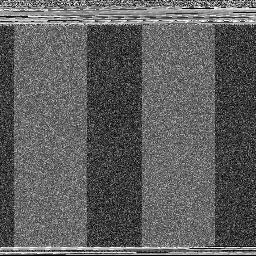
\includegraphics[width=.5\linewidth]{./imgs/MalwareSample/2/01IsoiSMh5gxyDYTl4CB.jpg}
  \caption{01IsoiSMh5gxyDYTl4CB}
\end{subfigure}%
\begin{subfigure}{.5\textwidth}
  \centering
  
\includegraphics[width=.5\linewidth]{./imgs/MalwareSample/2/02zcUmKV16Lya5xqnPGB.jpg}
  \caption{02zcUmKV16Lya5xqnPGB}
\end{subfigure}
\begin{subfigure}{.5\textwidth}
  \centering
  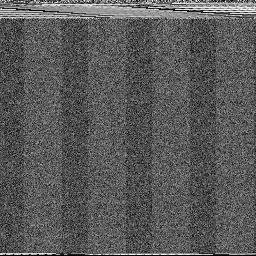
\includegraphics[width=.5\linewidth]{./imgs/MalwareSample/2/2ZNUOyAMv67lcYPoetkR.jpg}
  \caption{2ZNUOyAMv67lcYPoetkR}
\end{subfigure}
\begin{subfigure}{.5\textwidth}
  \centering
  
\includegraphics[width=.5\linewidth]{./imgs/MalwareSample/2/40ofYnDCl8TKJXwyGmrP.jpg}
  \caption{40ofYnDCl8TKJXwyGmrP}
\end{subfigure}
\caption{Sample Malware Images for Lollipop}
\label{malware image lollipop}
\end{figure}

\hspace{1pt}
\newline

\begin{figure}[ht!]
\begin{subfigure}{.5\textwidth}
  \centering
  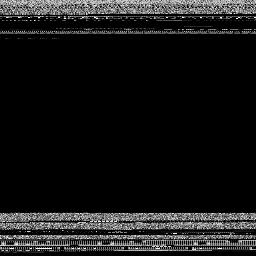
\includegraphics[width=.5\linewidth]{./imgs/MalwareSample/8/0AguvpOCcaf2myVDYFGb.jpg}
  \caption{0AguvpOCcaf2myVDYFGb}
\end{subfigure}%
\begin{subfigure}{.5\textwidth}
  \centering
  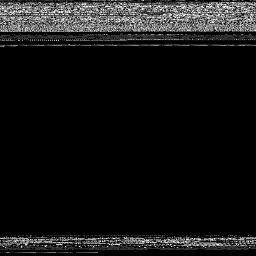
\includegraphics[width=.5\linewidth]{./imgs/MalwareSample/8/2TaBCxc4msyVU5YDRuOd.jpg}
  \caption{2TaBCxc4msyVU5YDRuOd}
\end{subfigure}
\begin{subfigure}{.5\textwidth}
  \centering
  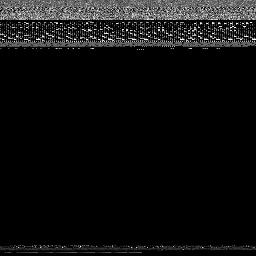
\includegraphics[width=.5\linewidth]{./imgs/MalwareSample/8/6jCs7bHULZXW3kKtxNRw.jpg}
  \caption{6jCs7bHULZXW3kKtxNRw}
\end{subfigure}
\begin{subfigure}{.5\textwidth}
  \centering
  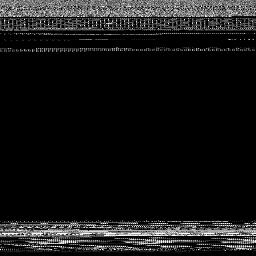
\includegraphics[width=.5\linewidth]{./imgs/MalwareSample/8/8lTjbp3rnwtLh104E57v.jpg}
  \caption{8lTjbp3rnwtLh104E57v}
\end{subfigure}
\caption{Sample Malware Images for Obfuscator.ACY}
\label{malware image Obfuscator}
\end{figure}

\clearpage

\begin{figure}[p!]
\centering
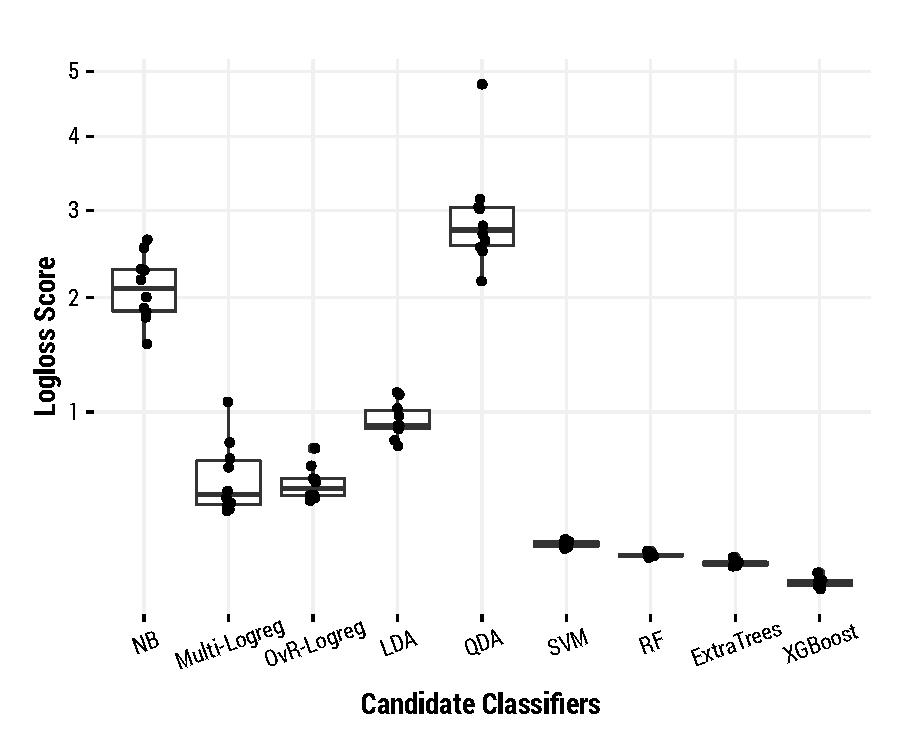
\includegraphics[width=1\linewidth]{./imgs/logloss.pdf}
\caption{Model Evaluation: Multi-Class Logloss}
\label{logloss}
\end{figure}

\begin{figure}[p!]
\centering
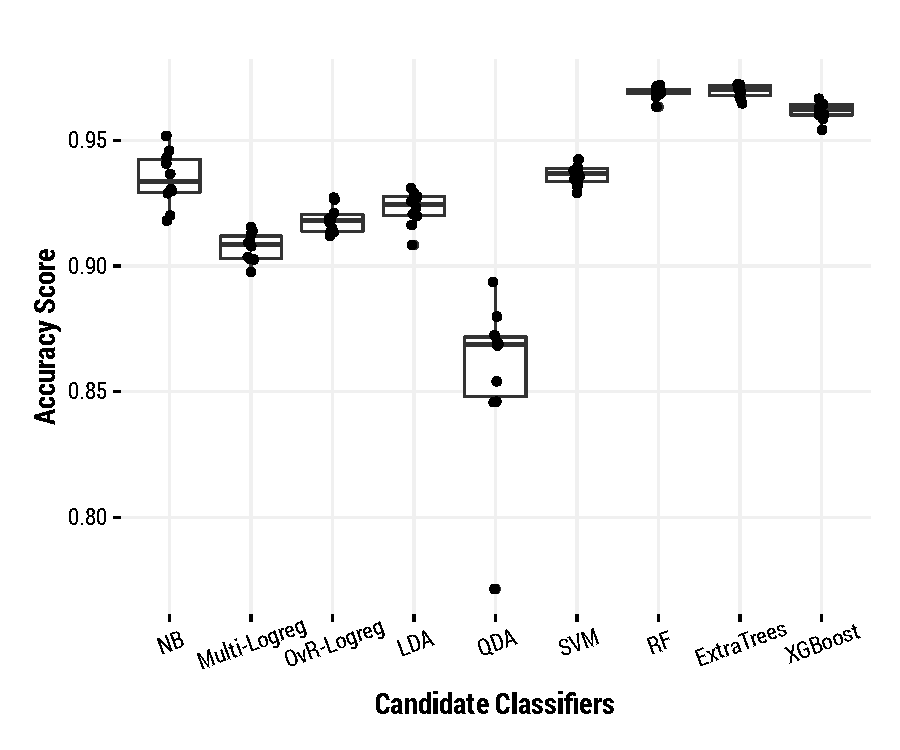
\includegraphics[width=1\linewidth]{./imgs/acc.pdf}
\caption{Model Evaluation: Multi-Class Accuracy}
\label{acc}
\end{figure}

\begin{figure}[p!]
\centering
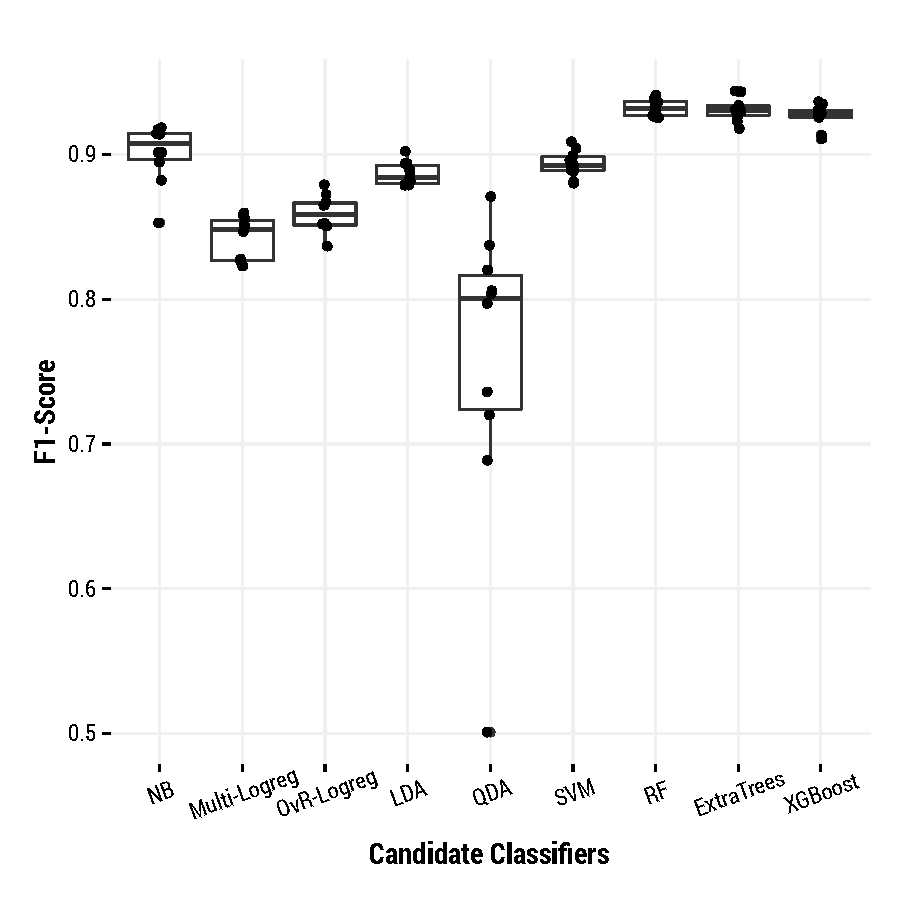
\includegraphics[width=1\linewidth]{./imgs/fscore0.pdf}
\caption{Model Evaluation: $F_{1}$ for Ramnit}
\label{f1, 0}
\end{figure}

\begin{figure}[p!]
\centering
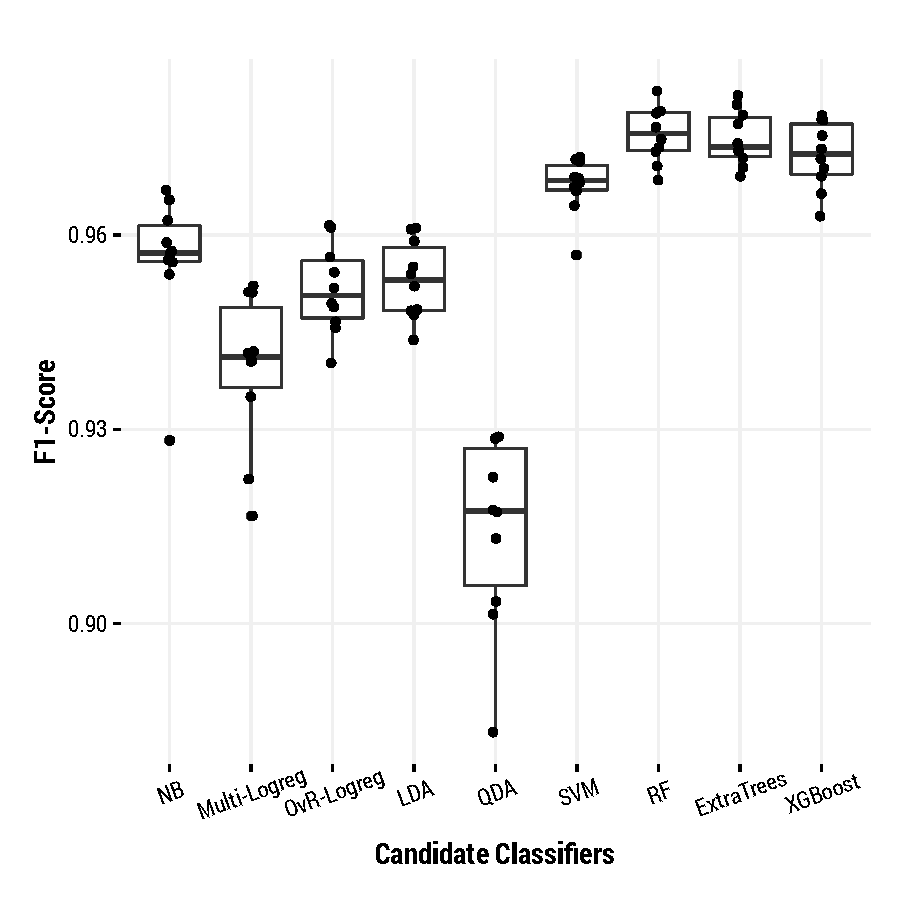
\includegraphics[width=1\linewidth]{./imgs/fscore1.pdf}
\caption{Model Evaluation: $F_{1}$ for Lollipop}
\label{f1, 1}
\end{figure}

\begin{figure}[p!]
\centering
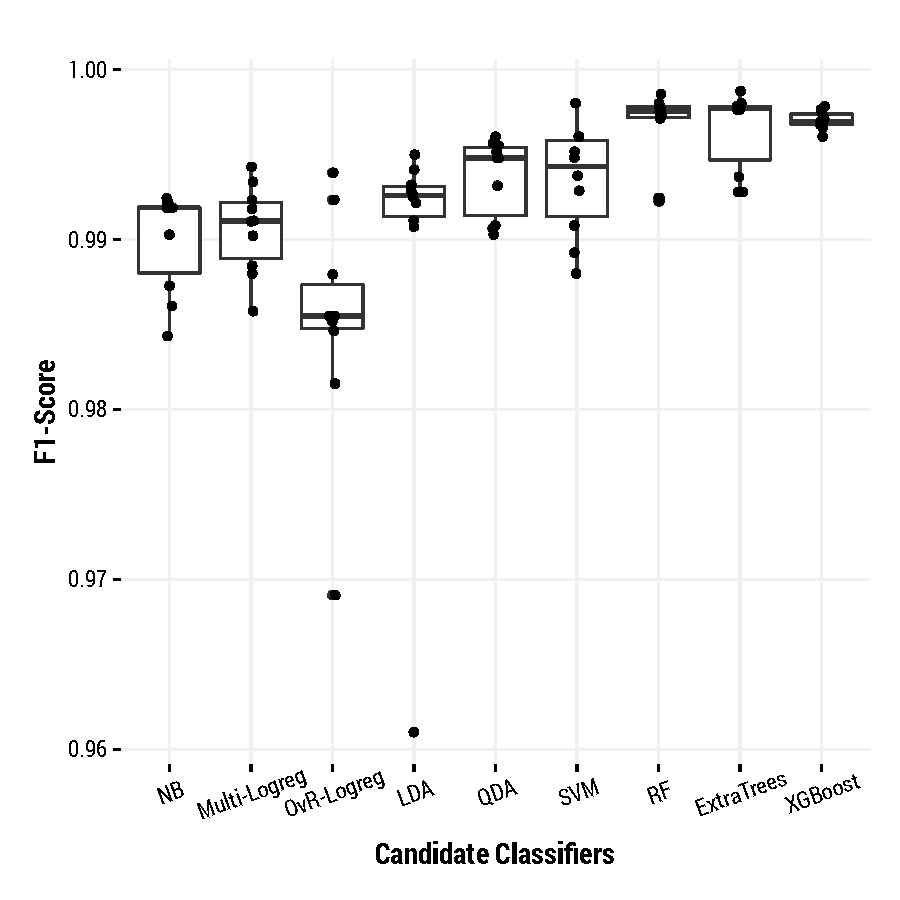
\includegraphics[width=1\linewidth]{./imgs/fscore2.pdf}
\caption{Model Evaluation: $F_{1}$ for Kelihos\_ver3}
\label{f1, 2}
\end{figure}

\begin{figure}[p!]
\centering
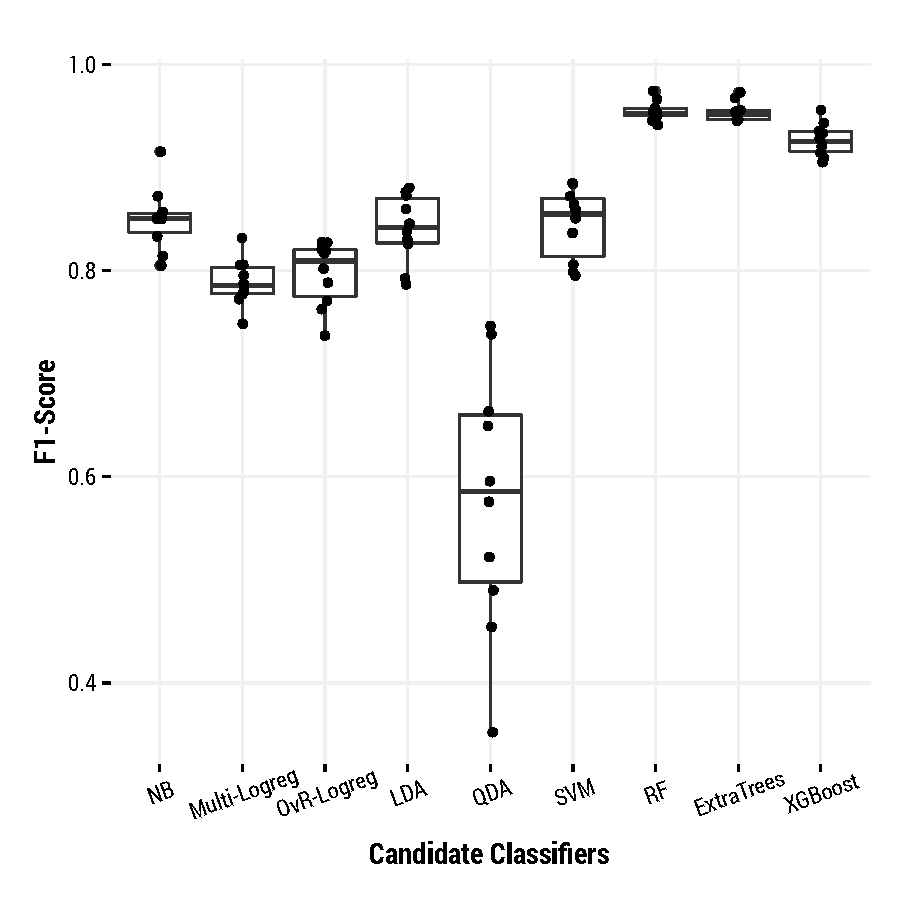
\includegraphics[width=1\linewidth]{./imgs/fscore3.pdf}
\caption{Model Evaluation: $F_{1}$ for Vundo}
\label{f1, 3}
\end{figure}


\begin{figure}[p!]
\centering
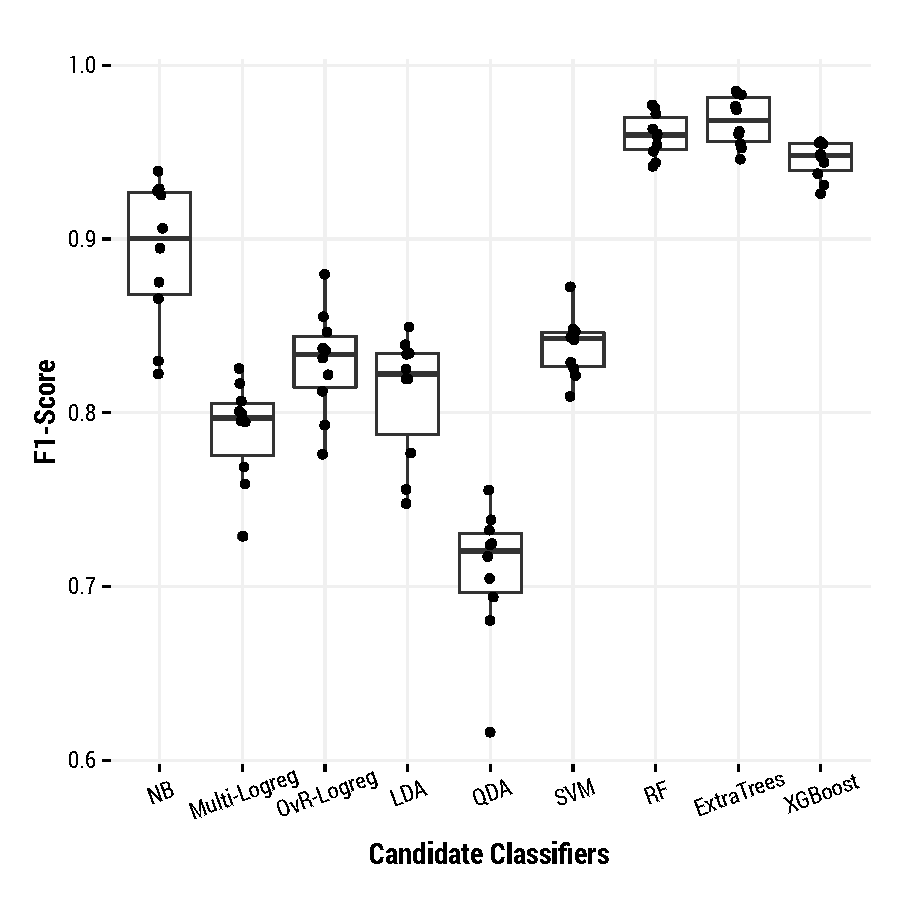
\includegraphics[width=1\linewidth]{./imgs/fscore4.pdf}
\caption{Model Evaluation: $F_{1}$ for Tracur}
\label{f1, 4}
\end{figure}


\begin{figure}[p!]
\centering
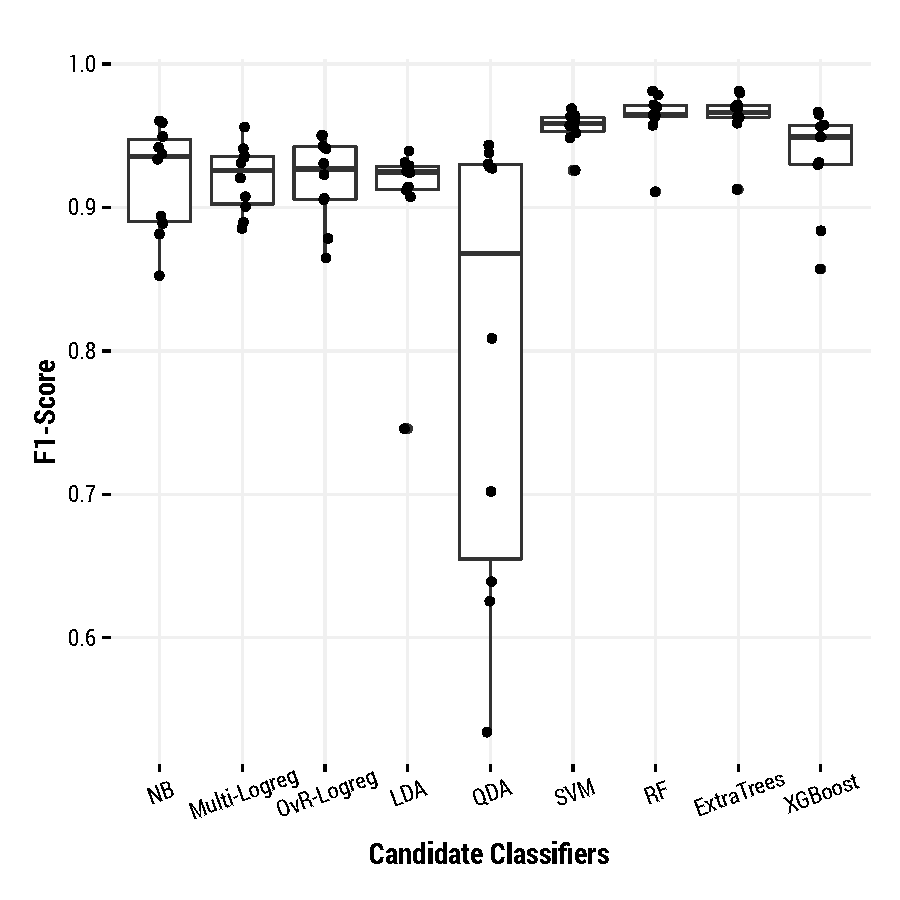
\includegraphics[width=1\linewidth]{./imgs/fscore5.pdf}
\caption{Model Evaluation: $F_{1}$ for Kelihos\_ver1}
\label{f1, 5}
\end{figure}


\begin{figure}[p!]
\centering
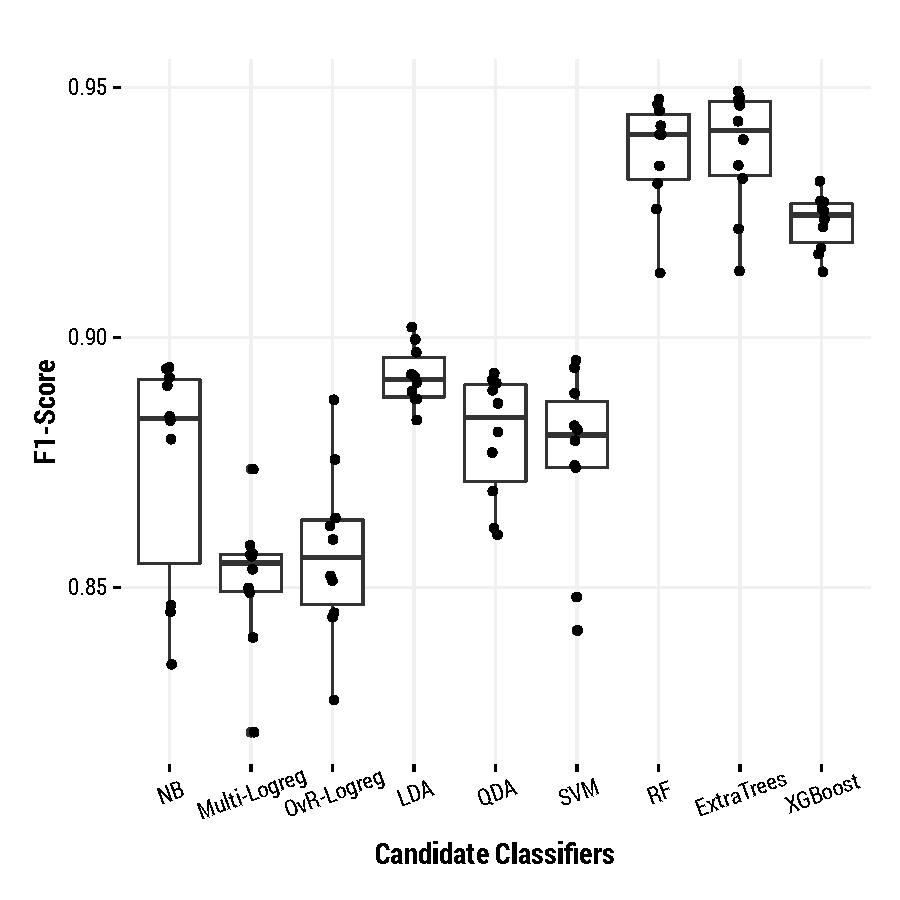
\includegraphics[width=1\linewidth]{./imgs/fscore6.pdf}
\caption{Model Evaluation: $F_{1}$ for Obfuscator.ACY}
\label{f1, 6}
\end{figure}


\begin{figure}[p!]
\centering
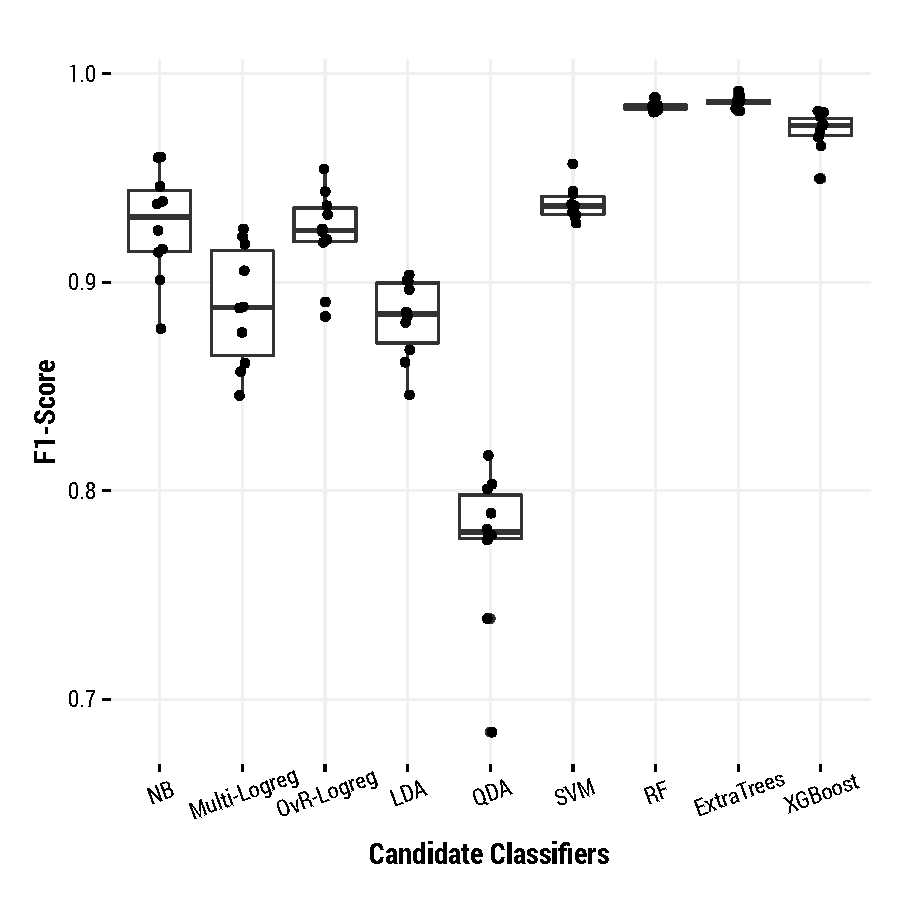
\includegraphics[width=1\linewidth]{./imgs/fscore7.pdf}
\caption{Model Evaluation: $F_{1}$ for Gatak}
\label{f1, 7}
\end{figure}


\clearpage
\begin{landscape}
\begin{table}[htbp]
\centering
\caption{Model Evaluation, Part 1}
\begin{tabular}{l|cc|ccc|ccc|ccc|ccc}
\toprule
 \multicolumn{1}{c}{  } & \multicolumn{2}{c}{Multi-Class}  & \multicolumn{3}{c}{ Ramnit } & \multicolumn{3}{c}{ Lollipop }  & \multicolumn{3}{c}{ Kelihos\_ver3 }  & \multicolumn{3}{c}{ Vundo }  \\
  & Logloss & Acc & Rec & Prec & F1 & Rec & Prec & F1 & Rec & Prec & F1 & Rec & Prec & F1 \\
\midrule
 \multirow{2}{*}{NB} & $2.11$ & $0.94$ & $0.94$ & $0.86$ & $0.90$ & $0.94$ & $0.97$ & $0.96$ & $0.98$ & $1.00$ & $0.99$ & $0.94$ & $0.78$ & $0.85$ \\
  & (0.33) & (0.01) & (0.01) & (0.04) & (0.02) & (0.02) & (0.01) & (0.01) & (0.00) & (0.00) & (0.00) & (0.02) & (0.06) & (0.03) \\
\midrule
 \multirow{2}{*}{Multi-Logreg} & $0.59$ & $0.91$ & $0.82$ & $0.87$ & $0.84$ & $0.94$ & $0.94$ & $0.94$ & $1.00$ & $0.99$ & $0.99$ & $0.78$ & $0.80$ & $0.79$ \\
  & (0.20) & (0.01) & (0.03) & (0.02) & (0.01) & (0.01) & (0.01) & (0.01) & (0.00) & (0.00) & (0.00) & (0.04) & (0.03) & (0.02) \\
\midrule
 \multirow{2}{*}{OvR-Logreg} & $0.55$ & $0.92$ & $0.85$ & $0.87$ & $0.86$ & $0.96$ & $0.95$ & $0.95$ & $1.00$ & $0.97$ & $0.99$ & $0.79$ & $0.81$ & $0.80$ \\
  & (0.09) & (0.01) & (0.02) & (0.03) & (0.00) & (0.01) & (0.01) & (0.01) & (0.00) & (0.01) & (0.01) & (0.06) & (0.05) & (0.03) \\
\midrule
 \multirow{2}{*}{LDA} & $0.94$ & $0.92$ & $0.89$ & $0.89$ & $0.89$ & $0.94$ & $0.97$ & $0.95$ & $0.99$ & $0.99$ & $0.99$ & $0.88$ & $0.81$ & $0.84$ \\
  & (0.12) & (0.01) & (0.02) & (0.02) & (0.01) & (0.01) & (0.01) & (0.01) & (0.02) & (0.00) & (0.01) & (0.05) & (0.04) & (0.03) \\
\midrule
 \multirow{2}{*}{QDA} & $2.94$ & $0.86$ & $0.70$ & $0.87$ & $0.76$ & $0.95$ & $0.88$ & $0.92$ & $0.99$ & $1.00$ & $0.99$ & $0.92$ & $0.44$ & $0.58$ \\
  & (0.68) & (0.03) & (0.16) & (0.05) & (0.10) & (0.02) & (0.03) & (0.01) & (0.00) & (0.00) & (0.00) & (0.04) & (0.13) & (0.12) \\
\midrule
 \multirow{2}{*}{SVM} & $0.27$ & $0.94$ & $0.93$ & $0.86$ & $0.89$ & $0.96$ & $0.98$ & $0.97$ & $1.00$ & $0.99$ & $0.99$ & $0.85$ & $0.84$ & $0.85$ \\
  & (0.01) & (0.00) & (0.03) & (0.02) & (0.01) & (0.01) & (0.01) & (0.00) & (0.01) & (0.00) & (0.00) & (0.06) & (0.05) & (0.03) \\
\midrule
 \multirow{2}{*}{RF} & $0.23$ & $\textbf{0.97}$ & $0.96$ & $0.90$ & $\textbf{0.93}$ & $0.99$ & $0.96$ & $0.98$ & $1.00$ & $1.00$ & $1.00$ & $0.96$ & $0.96$ & $0.96$ \\
  & (0.01) & (0.00) & (0.01) & (0.01) & (0.01) & (0.00) & (0.01) & (0.00) & (0.00) & (0.00) & (0.00) & (0.02) & (0.03) & (0.01) \\
\midrule
 \multirow{2}{*}{ExtraTrees} & $\textbf{0.20}$ & $\textbf{0.97}$ & $0.97$ & $0.90$ & $\textbf{0.93}$ & $0.99$ & $0.96$ & $0.98$ & $0.99$ & $1.00$ & $1.00$ & $0.96$ & $0.95$ & $0.95$ \\
  & (0.01) & (0.00) & (0.01) & (0.01) & (0.01) & (0.00) & (0.01) & (0.00) & (0.00) & (0.00) & (0.00) & (0.02) & (0.03) & (0.01) \\
\midrule
 \multirow{2}{*}{XGBoost} & $\textbf{0.14}$ & $0.96$ & $0.94$ & $0.91$ & $\textbf{0.93}$ & $0.98$ & $0.96$ & $0.97$ & $1.00$ & $1.00$ & $1.00$ & $0.95$ & $0.91$ & $0.93$ \\
  & (0.01) & (0.00) & (0.01) & (0.01) & (0.01) & (0.01) & (0.01) & (0.01) & (0.00) & (0.00) & (0.00) & (0.03) & (0.04) & (0.02) \\
\bottomrule
\end{tabular}
\label{model evaluation 1}
\end{table}
\end{landscape}

\clearpage
\begin{landscape}
\begin{table}[htbp]
\centering
\caption{Model Evaluation, Part 2}
\begin{tabular}{l|ccc|ccc|ccc|ccc}
\toprule
 \multicolumn{1}{c}{  } & \multicolumn{3}{c}{ Tracur } & \multicolumn{3}{c}{ Kelihos\_ver1 } & \multicolumn{3}{c}{ Obfuscator.ACY }  & \multicolumn{3}{c}{ Gatak } \\
& Rec & Prec & F1 & Rec & Prec & F1 & Rec & Prec & F1 & Rec & Prec & F1 \\
\midrule
 \multirow{2}{*}{NB} & $0.95$ & $0.84$ & $0.89$ & $0.89$ & $0.96$ & $0.92$ & $0.79$ & $0.98$ & $0.87$ & $0.94$ & $0.92$ & $0.93$ \\
  & (0.02) & (0.07) & (0.04) & (0.06) & (0.04) & (0.04) & (0.04) & (0.01) & (0.02) & (0.03) & (0.04) & (0.03) \\
\midrule
 \multirow{2}{*}{Multi-Logreg} & $0.78$ & $0.80$ & $0.79$ & $0.94$ & $0.90$ & $0.92$ & $0.85$ & $0.86$ & $0.85$ & $0.91$ & $0.87$ & $0.89$ \\
  & (0.04) & (0.04) & (0.03) & (0.01) & (0.05) & (0.02) & (0.01) & (0.02) & (0.01) & (0.03) & (0.05) & (0.03) \\
\midrule
 \multirow{2}{*}{OvR-Logreg} & $0.82$ & $0.84$ & $0.83$ & $0.91$ & $0.93$ & $0.92$ & $0.83$ & $0.89$ & $0.86$ & $0.94$ & $0.90$ & $0.92$ \\
  & (0.03) & (0.04) & (0.03) & (0.05) & (0.03) & (0.03) & (0.02) & (0.03) & (0.02) & (0.01) & (0.04) & (0.02) \\
\midrule
 \multirow{2}{*}{LDA} & $0.82$ & $0.81$ & $0.81$ & $0.93$ & $0.89$ & $0.91$ & $0.85$ & $0.94$ & $0.89$ & $0.94$ & $0.83$ & $0.88$ \\
  & (0.03) & (0.06) & (0.03) & (0.02) & (0.09) & (0.05) & (0.01) & (0.02) & (0.01) & (0.02) & (0.03) & (0.02) \\
\midrule
 \multirow{2}{*}{QDA} & $0.60$ & $0.87$ & $0.71$ & $0.95$ & $0.72$ & $0.80$ & $0.80$ & $0.98$ & $0.88$ & $0.67$ & $0.92$ & $0.78$ \\
  & (0.06) & (0.06) & (0.04) & (0.01) & (0.22) & (0.15) & (0.02) & (0.01) & (0.01) & (0.05) & (0.04) & (0.04) \\
\midrule
 \multirow{2}{*}{SVM} & $0.80$ & $0.88$ & $0.84$ & $0.94$ & $0.97$ & $0.96$ & $0.87$ & $0.89$ & $0.88$ & $0.94$ & $0.94$ & $0.94$ \\
  & (0.03) & (0.03) & (0.02) & (0.01) & (0.02) & (0.01) & (0.03) & (0.05) & (0.02) & (0.02) & (0.02) & (0.01) \\
\midrule
 \multirow{2}{*}{RF} & $0.96$ & $0.96$ & $0.96$ & $0.94$ & $0.99$ & $0.96$ & $0.90$ & $0.98$ & $0.94$ & $0.98$ & $0.99$ & $0.98$ \\
  & (0.02) & (0.02) & (0.01) & (0.01) & (0.03) & (0.02) & (0.02) & (0.01) & (0.01) & (0.01) & (0.00) & (0.00) \\
\midrule
 \multirow{2}{*}{ExtraTrees} & $0.95$ & $0.98$ & $0.97$ & $0.94$ & $0.99$ & $0.96$ & $0.90$ & $0.98$ & $0.94$ & $0.98$ & $1.00$ & $0.99$ \\
  & (0.02) & (0.02) & (0.01) & (0.02) & (0.03) & (0.02) & (0.02) & (0.01) & (0.01) & (0.00) & (0.00) & (0.00) \\
\midrule
 \multirow{2}{*}{XGBoost} & $0.95$ & $0.95$ & $0.95$ & $0.91$ & $0.96$ & $0.94$ & $0.89$ & $0.95$ & $0.92$ & $0.97$ & $0.98$ & $0.97$ \\
  & (0.02) & (0.03) & (0.01) & (0.04) & (0.05) & (0.04) & (0.02) & (0.01) & (0.01) & (0.02) & (0.01) & (0.01) \\
\bottomrule
\end{tabular}
\label{model evaluation 2}
\end{table}
\end{landscape}
\end{document}
